\documentclass[Bachelorarbeit.tex]{subfiles}
\begin{document}

\graphicspath{{./figures/appendixResults/}}	%specifying the folder for the figures

\chapter{Results for Hub-Based, Scale-Free and Small-World}
\label{app:results}

\section{Half-Fully Connected}
\begin{figure}[H]
	\centering
  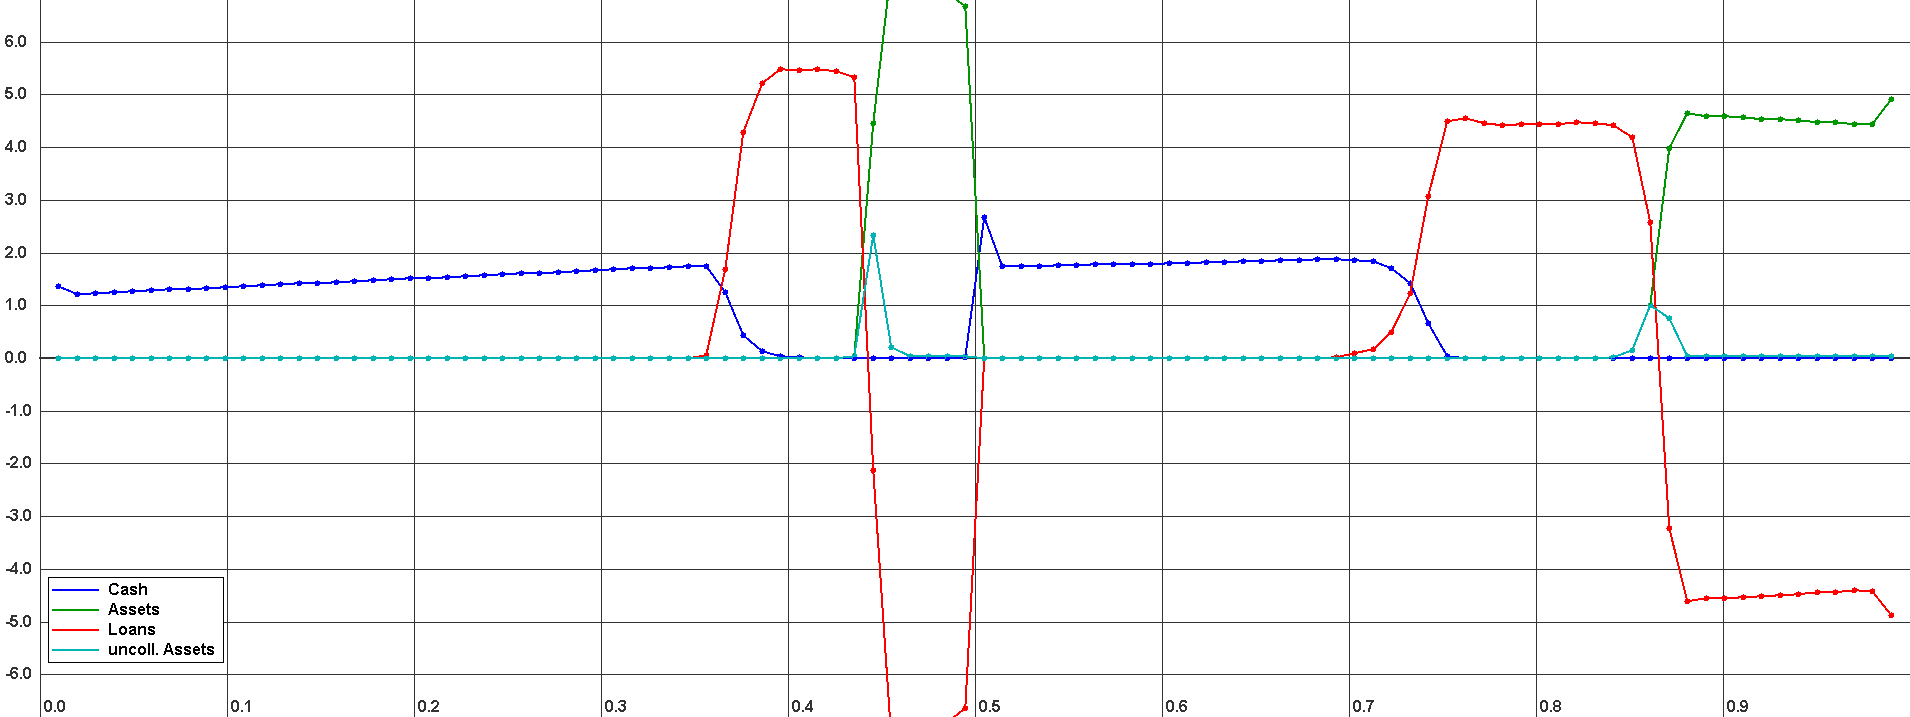
\includegraphics[width=1.0\textwidth, angle=0]{HALFFULLYCONNECTED_100_NOCOLLATERALMARKET_REPL.png}
	\caption{Wealth-Distribution of Half-Fully Connected topology }
	\label{fig:wealth_HALFFULLYCONNECTED_100_NOCOLLATERALMARKET_REPL}
\end{figure}

\begin{table}[H]
	\caption{Equilibrium of Half-Fully Connected topology}
	\centering
	\begin{tabular} { l c r }
		\hline
		Asset-Price p & 0.651 (0.027) \\
		Bond-Price q & 0.362 (0.013) \\
		Marginal agent i1 & 0.640 (0.015) \\
		Marginal agent i2 & 0.833 (0.09) \\
		\hline
		Pessimist Wealth & 1.22 (0.096) \\
		Medianist Wealth & 2.258 (0.409) \\
		Optimist Wealth & 4.526 (0.071) \\
		\hline
	\end{tabular}
\end{table} 

\begin{table}[H]
	\caption{Performance of Half-Fully Connected topology}
	\centering
	\begin{tabular} { l c r }
		\hline
		Successful matching-rounds& 14,218.9 (4621.74) \\
		Failed matching-rounds & 1034.12 (22.99) \\
		Total matching-rounds & 15,253.02 (4633.44) \\
		\hline
		Ratio successful/total & 0.93 \\
		Ratio failed/total & 0.07 \\
		\hline
	\end{tabular}
\end{table}

The equilibrium is clearly distinct from the theoretical and Fully-Connected one as miss-allocation can be found within the pessimists-range. Also the i1- and i2-points and the wealth-distributions differ both numerically and visually. 

\section{Ascending-Connected with short-cuts}
\label{app:results_acShortCuts}

\subsection{Random short-cuts}
\begin{figure}[H]
	\centering
  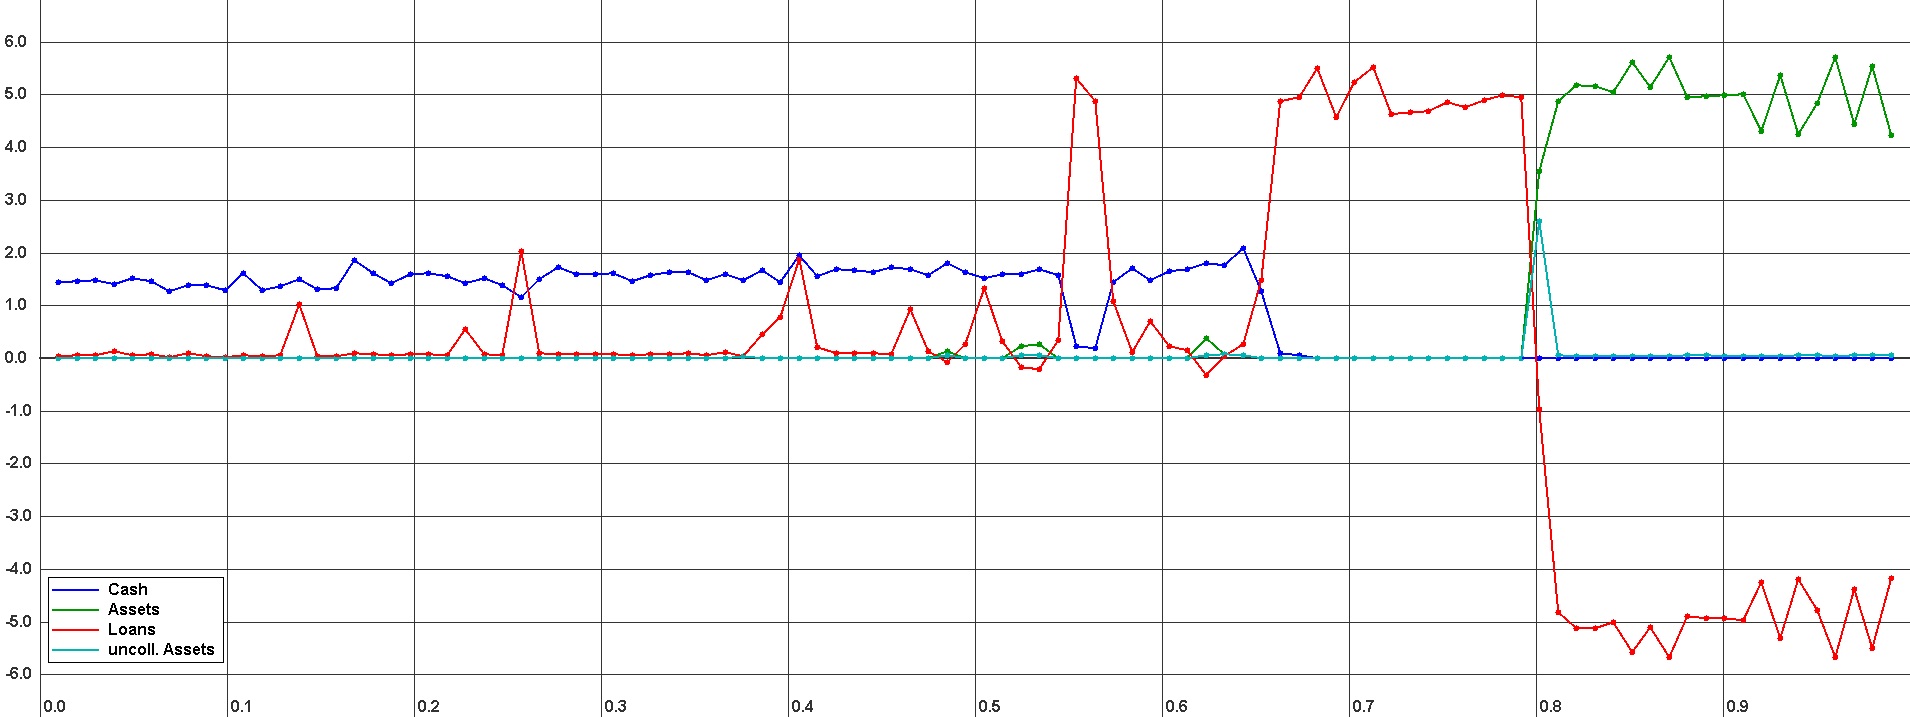
\includegraphics[width=1.0\textwidth, angle=0]{ASCENDINGCONNECTED_RANDSHORTCUTS_100_NOCOLLATERALMARKET_REPL.png}
	\caption{Wealth-Distribution of Ascending-Connected random short-cuts topology}
	\label{fig:wealth_ASCENDINGCONNECTED_RANDSHORTCUTS_100_NOCOLLATERALMARKET_REPL}
\end{figure}

\begin{table}[H]
	\caption{Equilibrium of Ascending-Connected random short-cuts topology}
	\centering
	\begin{tabular} { l c r }
		\hline
		Asset-Price p & 0.731 (0.019) \\
		Bond-Price q & 0.393 (0.009) \\
		Marginal agent i1 & 0.649 (0.005) \\
		Marginal agent i2 & 0.804 (0.004) \\
		\hline
		Pessimist Wealth & 1.441 (0.03) \\
		Medianist Wealth & 4.282 (0.278) \\
		Optimist Wealth & 4.974 (0.038) \\
		\hline
	\end{tabular}
\end{table} 

\begin{table}[H]
	\caption{Performance of Ascending-Connected random short-cuts topology}
	\centering
	\begin{tabular} { l c r }
		\hline
		Successful matching-rounds& 8314.78 (229.85) \\
		Failed matching-rounds & 1182.06 (29.23) \\
		Total matching-rounds & 9496.84 (228.23) \\
		\hline
		Ratio successful/total & 0.87 \\
		Ratio failed/total & 0.13 \\
		\hline
	\end{tabular}
\end{table}

Random short-cuts seem to reduce the miss-allocation of pessimists-wealth a bit but lead to a fundamental different equilibrium than the theoretical or fully-connected one as can clearly be seen both visually and numerically.

\subsection{2 short-cuts}
\begin{figure}[H]
	\centering
  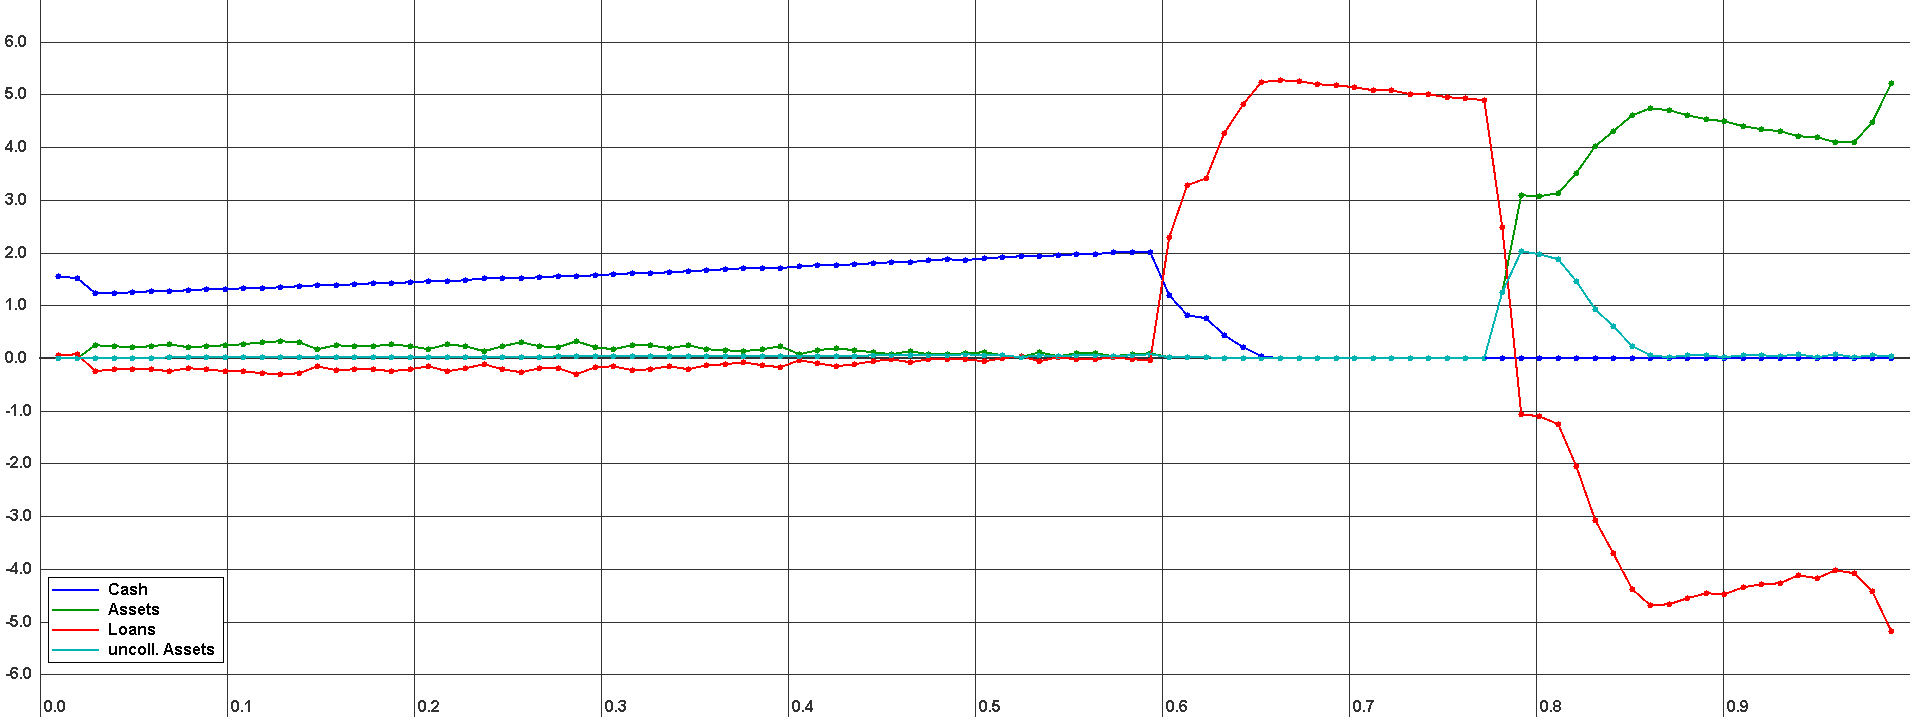
\includegraphics[width=1.0\textwidth, angle=0]{ASCENDINGCONNECTED_2SC_100_NOCOLLATERALMARKET_REPL.png}
	\caption{Wealth-Distribution of Ascending-Connected 2 short-cuts topology}
	\label{fig:wealth_ASCENDINGCONNECTED_2SC_100_NOCOLLATERALMARKET_REPL}
\end{figure}

\begin{table}[H]
	\caption{Equilibrium of Ascending-Connected 2 short-cuts topology}
	\centering
	\begin{tabular} { l c r }
		\hline
		Asset-Price p & 0.662 (0.024) \\
		Bond-Price q & 0.376 (0.006) \\
		Marginal agent i1 & 0.608 (0.018) \\
		Marginal agent i2 & 0.805 (0.028) \\
		\hline
		Pessimist Wealth & 1.441 (0.21) \\
		Medianist Wealth & 3.978 (1.442) \\
		Optimist Wealth & 4.514 (0.063) \\
		\hline
	\end{tabular}
\end{table} 

\begin{table}[H]
	\caption{Performance of Ascending-Connected random short-cuts topology}
	\centering
	\begin{tabular} { l c r }
		\hline
		Successful matching-rounds& 37,093.64 (12,864.4) \\
		Failed matching-rounds & 1021. (18.85) \\
		Total matching-rounds & 38,115.54 (12,851.53) \\
		\hline
		Ratio successful/total & 0.97 \\
		Ratio failed/total & 0.03 \\
		\hline
	\end{tabular}
\end{table}

This topology reduces the miss-allocation in the pessimists-range dramatically but doesn't solve it yet. Unfortunately it leads to a dramatically different wealth-distribution within the medianists and optimist.

\subsection{5 full short-cuts}
\begin{figure}[H]
	\centering
  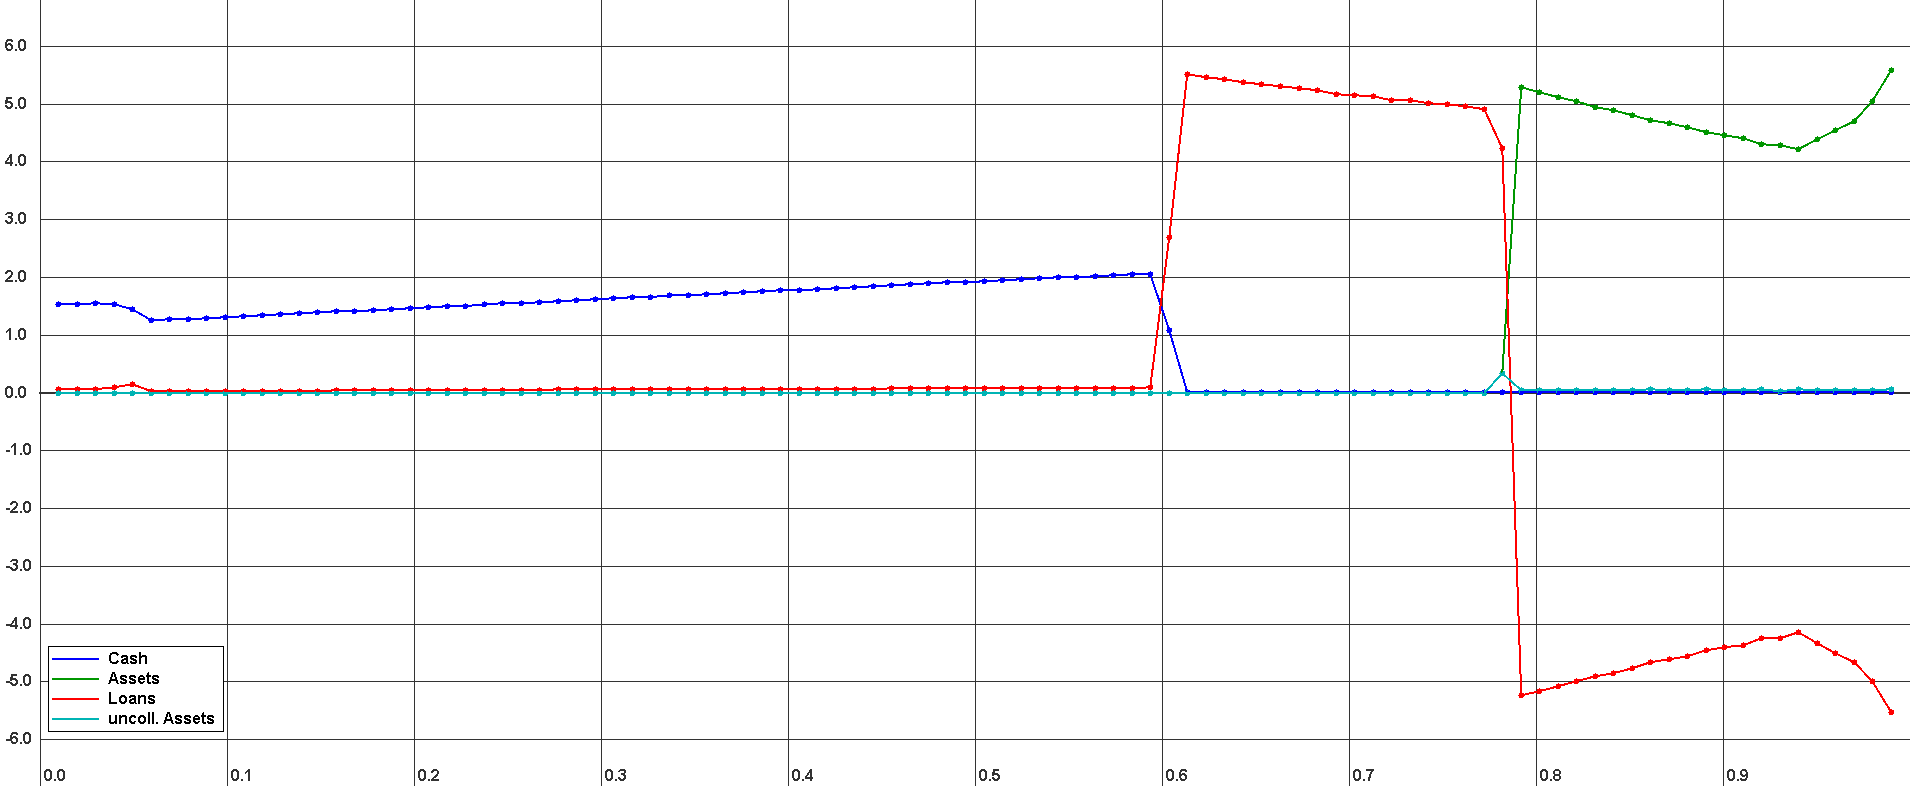
\includegraphics[width=1.0\textwidth, angle=0]{ASCENDINGCONNECTED_5FullSC_100_NOCOLLATERALMARKET_REPL.png}
	\caption{Wealth-Distribution of Ascending-Connected 5 full short-cuts topology}
	\label{fig:wealth_ASCENDINGCONNECTED_5FullSC_100_NOCOLLATERALMARKET_REPL}
\end{figure}

\begin{table}[H]
	\caption{Equilibrium of Ascending-Connected 5 full short-cuts}
	\centering
	\begin{tabular} { l c r }
		\hline
		Asset-Price p & 0.656 (0.019) \\
		Bond-Price q & 0.371 (0.003) \\
		Marginal agent i1 & 0.594 (0.0) \\
		Marginal agent i2 & 0.792 (0.0) \\
		\hline
		Pessimist Wealth & 1.649 (0.002) \\
		Medianist Wealth & 5.013 (0.018) \\
		Optimist Wealth & 4.746 (0.011) \\
		\hline
	\end{tabular}
\end{table} 

\begin{table}[H]
	\caption{Performance of Ascending-Connected 5 full short-cuts topology}
	\centering
	\begin{tabular} { l c r }
		\hline
		Successful matching-rounds& 16,971.34 (228.0) \\
		Failed matching-rounds & 1026.92 (22.68) \\
		Total matching-rounds & 17,998.26 (225.23) \\
		\hline
		Ratio successful/total & 0.94 \\
		Ratio failed/total & 0.06 \\
		\hline
	\end{tabular}
\end{table}

As can be clearly seen this topology seems to be able to solve miss-allocations in the pessimists-range seen in Ascending-Connected topology but is still different than the theoretical and Fully-Connected equilibrium.

\subsection{15 full short-cuts}
\begin{figure}[H]
	\centering
  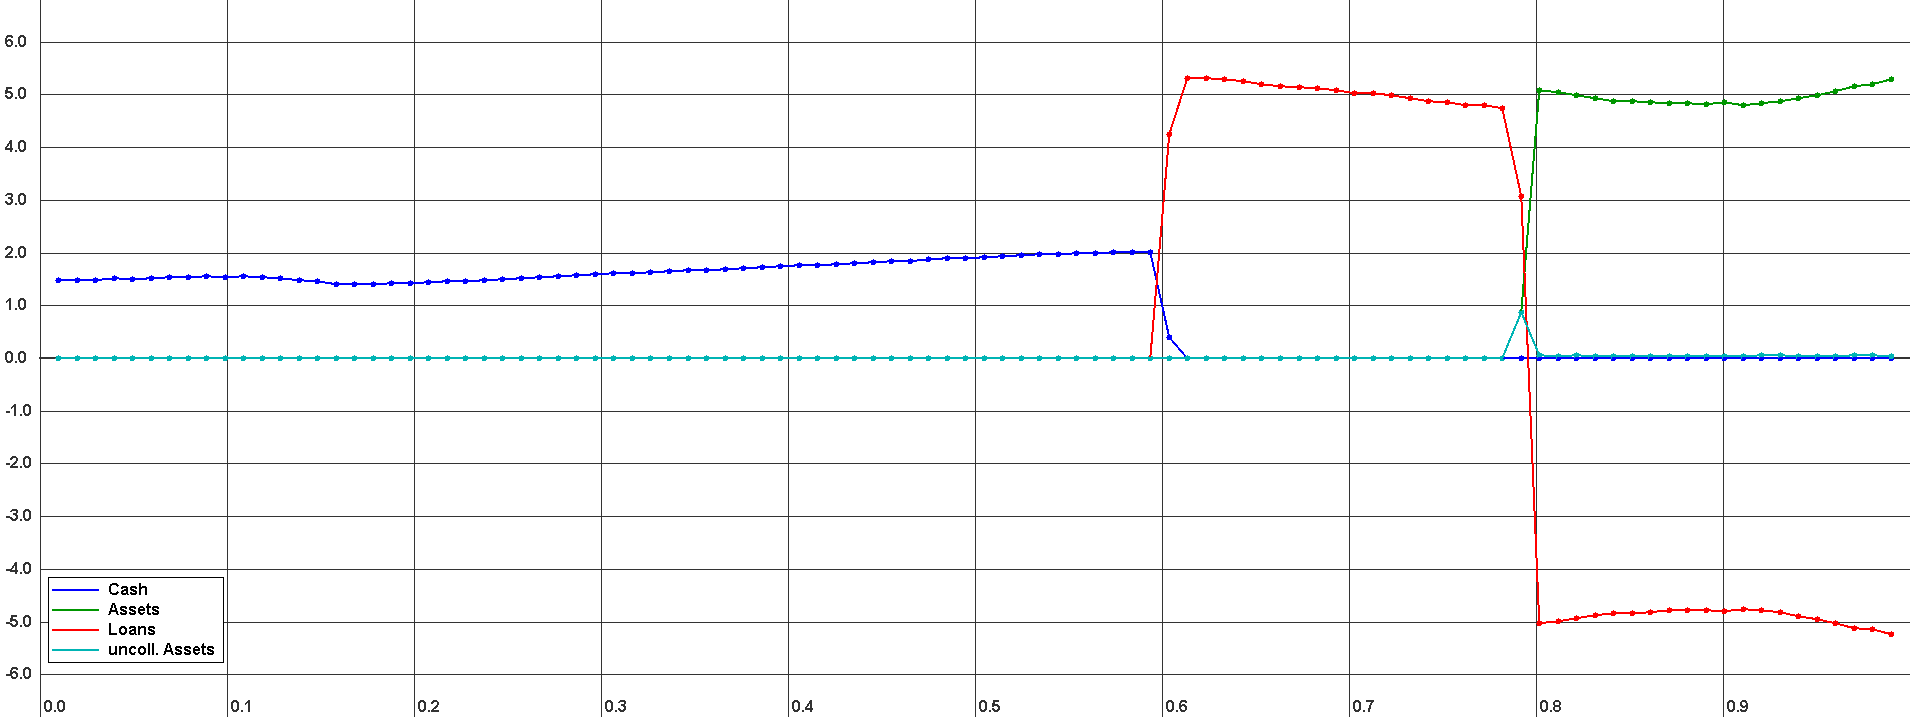
\includegraphics[width=1.0\textwidth, angle=0]{ASCENDINGCONNECTED_15FullSC_100_NOCOLLATERALMARKET_REPL.png}
	\caption{Wealth-Distribution of Ascending-Connected 15 full short-cuts topology}
	\label{fig:wealth_ASCENDINGCONNECTED_15FullSC_100_NOCOLLATERALMARKET_REPL}
\end{figure}

\begin{table}[H]
	\caption{Equilibrium of Ascending-Connected 15 full short-cuts topology}
	\centering
	\begin{tabular} { l c r }
		\hline
		Asset-Price p & 0.658 (0.024) \\
		Bond-Price q & 0.366 (0.009) \\
		Marginal agent i1 & 0.601 (0.004) \\
		Marginal agent i2 & 0.802 (0.0) \\
		\hline
		Pessimist Wealth & 1.649 (0.004) \\
		Medianist Wealth & 4.811 (0.092) \\
		Optimist Wealth & 4.957 (0.021) \\
		\hline
	\end{tabular}
\end{table} 

\begin{table}[H]
	\caption{Performance of Ascending-Connected 15 full short-cuts topology}
	\centering
	\begin{tabular} { l c r }
		\hline
		Successful matching-rounds& 4498.08 (58.67) \\
		Failed matching-rounds & 1024.78 (17.3) \\
		Total matching-rounds & 5522.860 (64.72) \\
		\hline
		Ratio successful/total & 0.81 \\
		Ratio failed/total & 0.19 \\
		\hline
	\end{tabular}
\end{table}

This topology comes very close to the theoretical equilibrium but is still a bit different as can be seen in the curved wealth-distributions of the pure optimists.

\subsection{30 full short-cuts}
\begin{figure}[H]
	\centering
  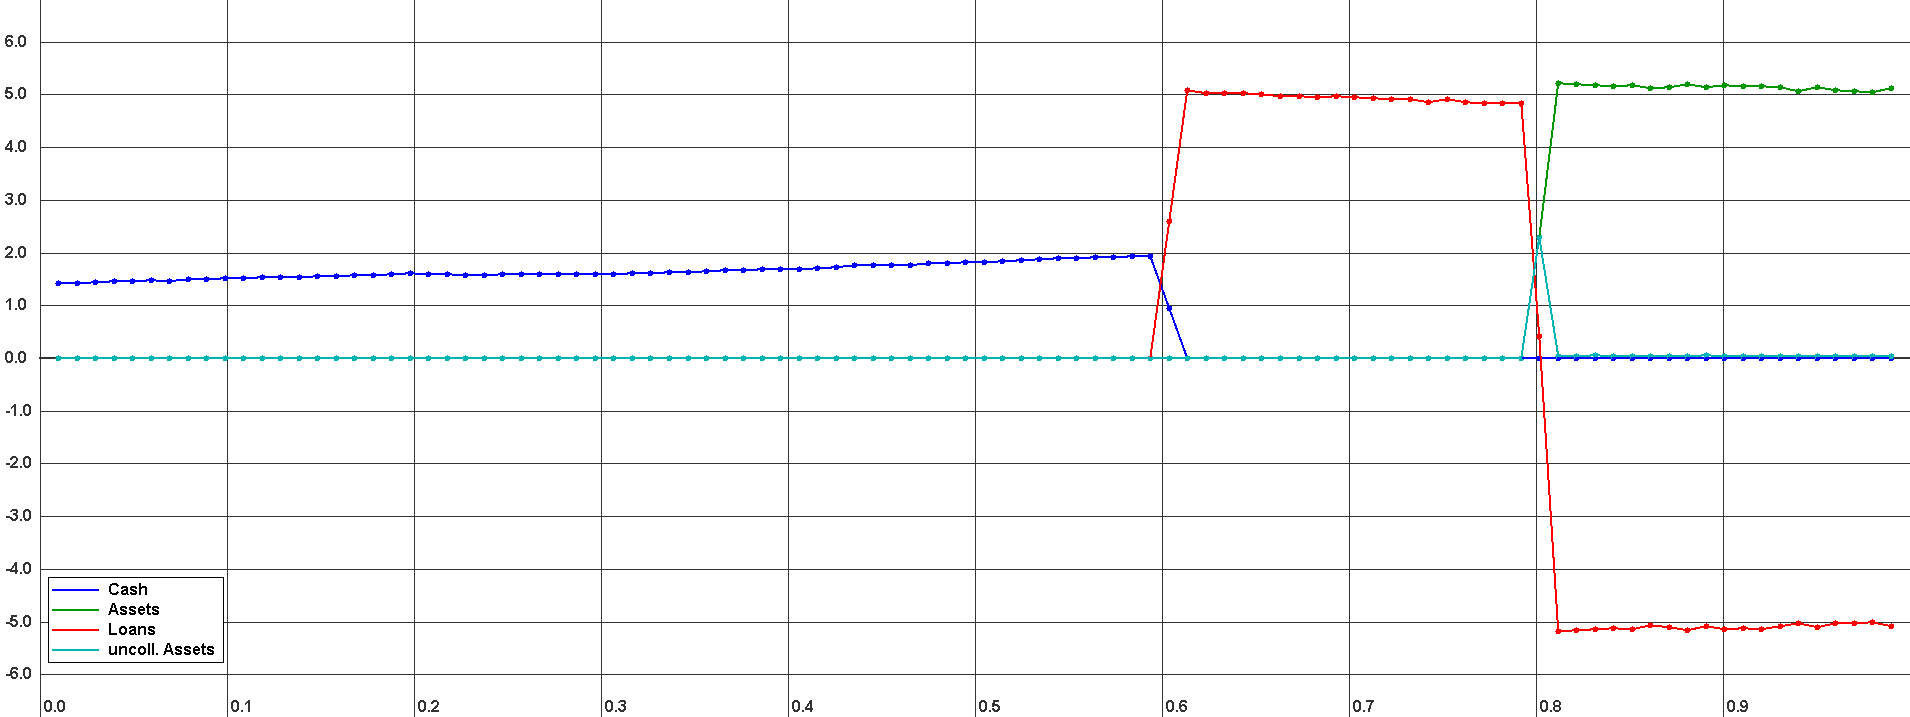
\includegraphics[width=1.0\textwidth, angle=0]{ASCENDINGCONNECTED_30FullSC_100_NOCOLLATERALMARKET_REPL.png}
	\caption{Wealth-Distribution of Ascending-Connected 30 full short-cuts topology}
	\label{fig:wealth_ASCENDINGCONNECTED_30FullSC_100_NOCOLLATERALMARKET_REPL}
\end{figure}

\begin{table}[H]
	\caption{Equilibrium of Ascending-Connected 30 full short-cuts topology}
	\centering
	\begin{tabular} { l c r }
		\hline
		Asset-Price p & 0.681 (0.012) \\
		Bond-Price q & 0.378 (0.006) \\
		Marginal agent i1 & 0.603 (0.006) \\
		Marginal agent i2 & 0.802 (0.1) \\
		\hline
		Pessimist Wealth & 1.649 (0.009) \\
		Medianist Wealth & 4.702 (0.112) \\
		Optimist Wealth & 5.004 (0.025) \\
		\hline
	\end{tabular}
\end{table} 

\begin{table}[H]
	\caption{Performance of Ascending-Connected 30 full short-cuts topology}
	\centering
	\begin{tabular} { l c r }
		\hline
		Successful matching-rounds& 2211.08 (35.88) \\
		Failed matching-rounds & 1014.68 (10.55) \\
		Total matching-rounds & 3225.76 (40.18) \\
		\hline
		Ratio successful/total & 0.68 \\
		Ratio failed/total & 0.32 \\
		\hline
	\end{tabular}
\end{table}

This topology is very close to the theoretical and Fully-Connected equilibrium although it differs in asset-price p and in the wealth-distributions. Of course with 30 fully short-cuts in a network of 100 agents one is already very close to fully connectedness.

\subsection{5 regular short-cuts}
\begin{figure}[H]
	\centering
  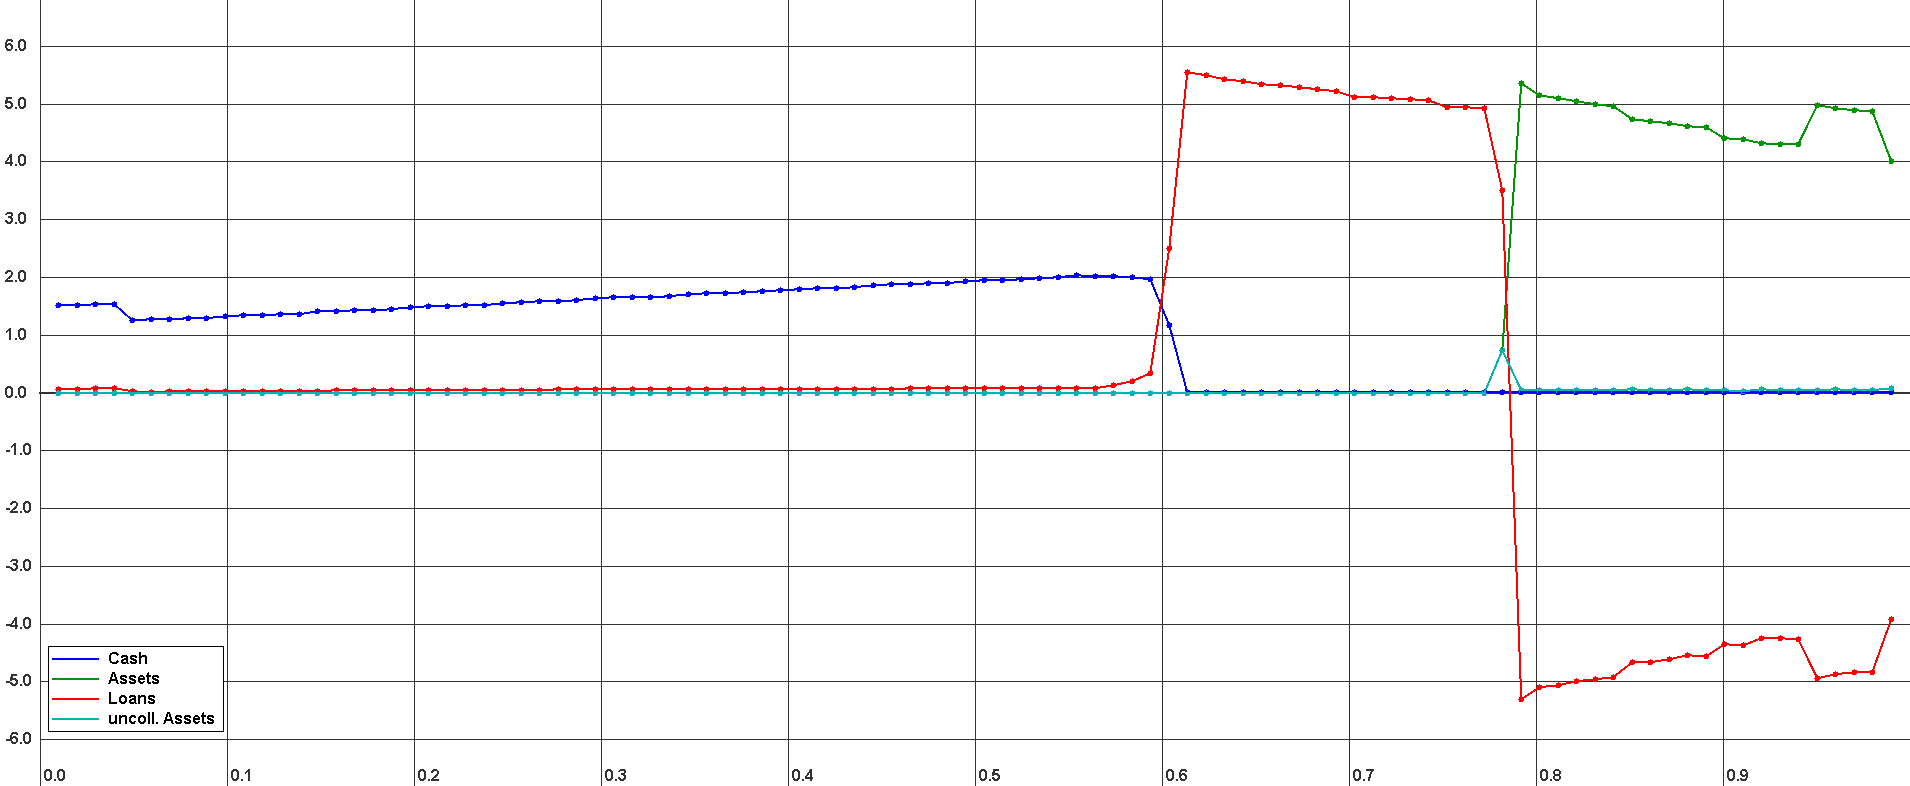
\includegraphics[width=1.0\textwidth, angle=0]{ASCENDINGCONNECTED_5RegSC_100_NOCOLLATERALMARKET_REPL.png}
	\caption{Wealth-Distribution of Ascending-Connected 5 regular short-cuts topology}
	\label{fig:wealth_ASCENDINGCONNECTED_5RegSC_100_NOCOLLATERALMARKET_REPL}
\end{figure}

\begin{table}[H]
	\caption{Equilibrium of Ascending-Connected 5 regular short-cuts topology}
	\centering
	\begin{tabular} { l c r }
		\hline
		Asset-Price p & 0.665 (0.016) \\
		Bond-Price q & 0.364 (0.007) \\
		Marginal agent i1 & 0.595 (0.003) \\
		Marginal agent i2 & 0.792 (0.0) \\
		\hline
		Pessimist Wealth & 1.649 (0.003) \\
		Medianist Wealth & 4.991 (0.045) \\
		Optimist Wealth & 4.727 (0.011) \\
		\hline
	\end{tabular}
\end{table} 

\begin{table}[H]
	\caption{Performance of Ascending-Connected 5 regular short-cuts topology}
	\centering
	\begin{tabular} { l c r }
		\hline
		Successful matching-rounds& 14,570.44 (157.61) \\
		Failed matching-rounds & 1064.24 (29.88) \\
		Total matching-rounds & 15,634.68 (166.21) \\
		\hline
		Ratio successful/total & 0.93 \\
		Ratio failed/total & 0.07 \\
		\hline
	\end{tabular}
\end{table}

As can be seen in the visual results this topology shows a different equilibrium than the theoretical and Fully-Connected one.

\subsection{15 regular short-cuts}
\begin{figure}[H]
	\centering
  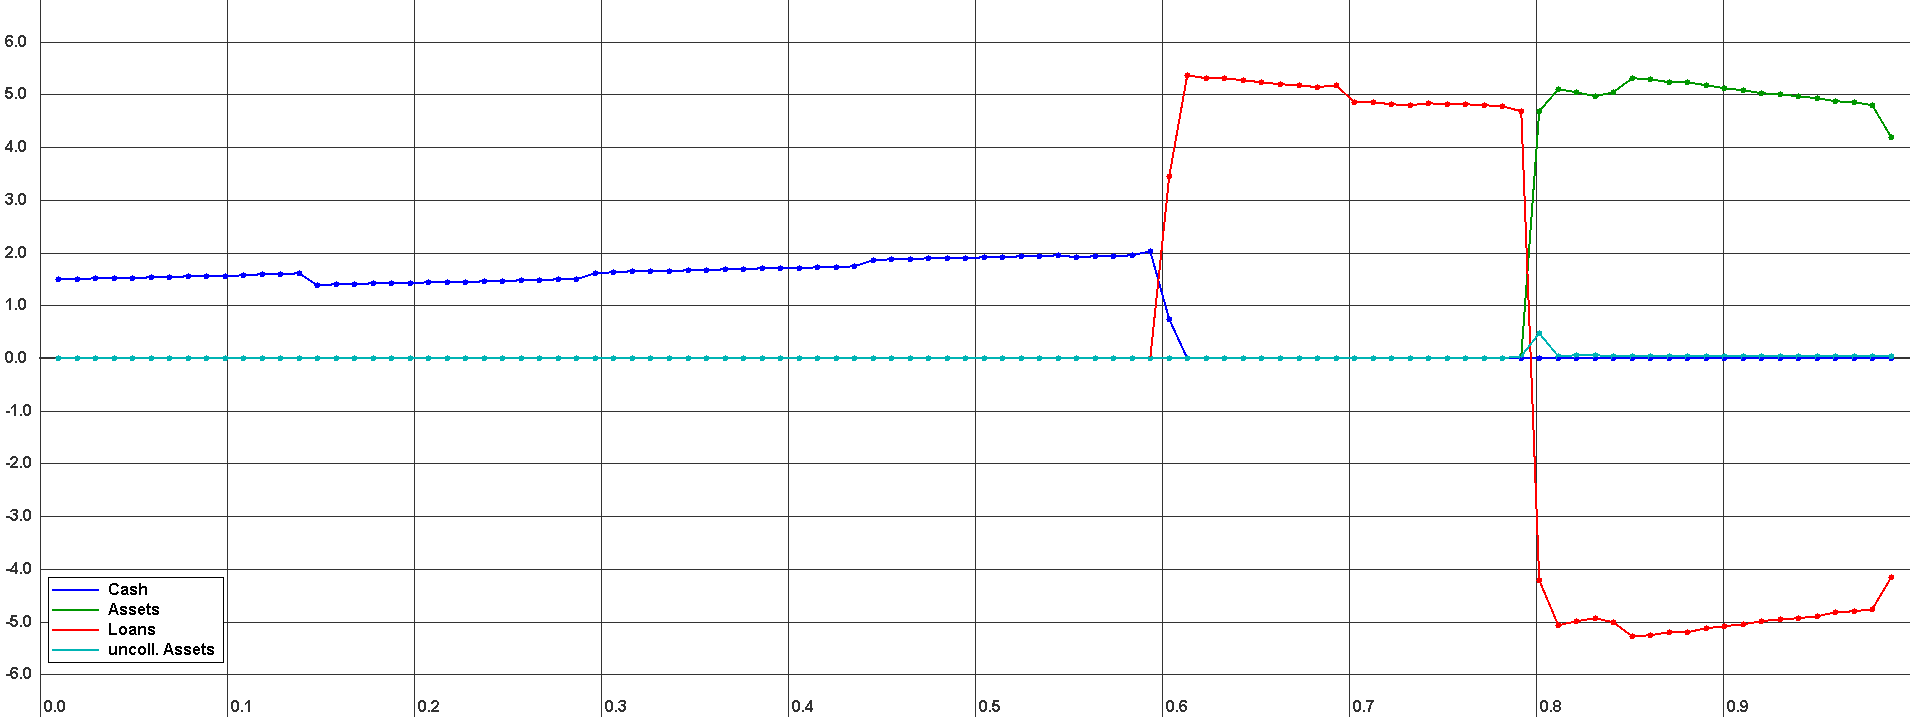
\includegraphics[width=1.0\textwidth, angle=0]{ASCENDINGCONNECTED_15RegSC_100_NOCOLLATERALMARKET_REPL.png}
	\caption{Wealth-Distribution of Ascending-Connected 15 regular short-cuts topology}
	\label{fig:wealth_ASCENDINGCONNECTED_15RegSC_100_NOCOLLATERALMARKET_REPL}
\end{figure}

\begin{table}[H]
	\caption{Equilibrium Ascending-Connected 15 regular short-cuts topology}
	\centering
	\begin{tabular} { l c r }
		\hline
		Asset-Price p & 0.705 (0.020) \\
		Bond-Price q & 0.357 (0.018) \\
		Marginal agent i1 & 0.586 (0.023) \\
		Marginal agent i2 & 0.802 (0.0) \\
		\hline
		Pessimist Wealth & 1.649 (0.051) \\
		Medianist Wealth & 4.146 (0.101) \\
		Optimist Wealth & 4.997 (0.007) \\
		\hline
	\end{tabular}
\end{table} 

\begin{table}[H]
	\caption{Performance of Ascending-Connected 15 regular short-cuts topology}
	\centering
	\begin{tabular} { l c r }
		\hline
		Successful matching-rounds& 4373.28 (50.13) \\
		Failed matching-rounds & 1129.24 (19.2) \\
		Total matching-rounds & 5502.52 (52.11) \\
		\hline
		Ratio successful/total & 0.79 \\
		Ratio failed/total & 0.21 \\
		\hline
	\end{tabular}
\end{table}

The equilibrium of this topology is falls very far from the theoretical and Fully-Connected one.

\subsection{30 regular short-cuts}
\begin{figure}[H]
	\centering
  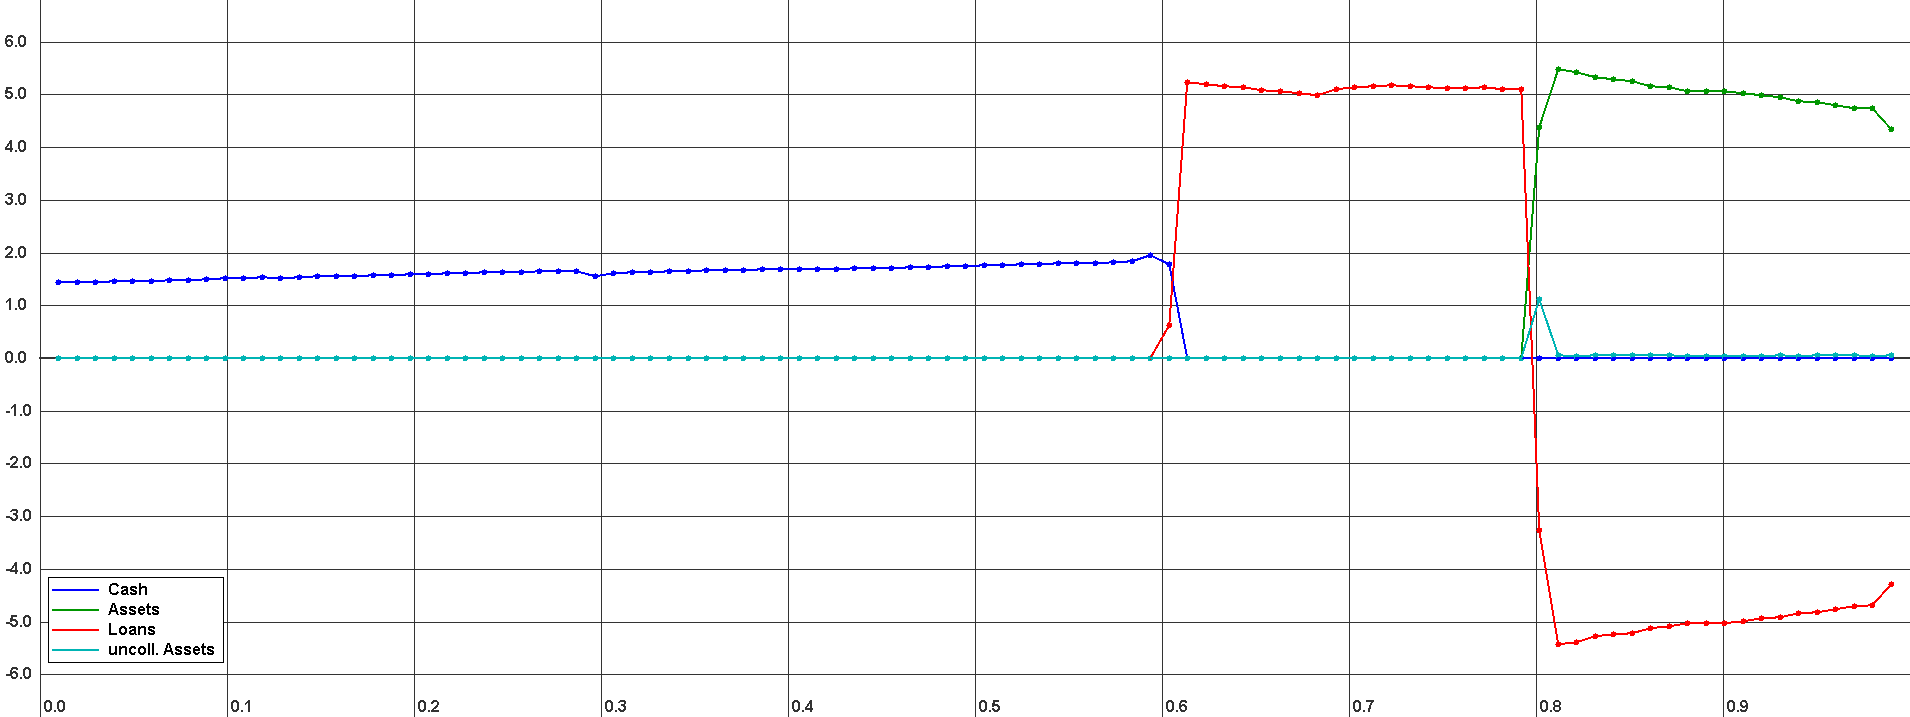
\includegraphics[width=1.0\textwidth, angle=0]{ASCENDINGCONNECTED_30RegSC_100_NOCOLLATERALMARKET_REPL.png}
	\caption{Wealth-Distribution of Ascending-Connected 30 regular short-cuts topology}
	\label{fig:wealth_ASCENDINGCONNECTED_30RegSC_100_NOCOLLATERALMARKET_REPL}
\end{figure}

\begin{table}[H]
	\caption{Equilibrium of Ascending-Connected 30 regular short-cuts topology}
	\centering
	\begin{tabular} { l c r }
		\hline
		Asset-Price p & 0.710 (0.021) \\
		Bond-Price q & 0.398 (0.008) \\
		Marginal agent i1 & 0.589 (0.021) \\
		Marginal agent i2 & 0.802 (0.0) \\
		\hline
		Pessimist Wealth & 1.479 (0.049) \\
		Medianist Wealth & 3.713 (0.125) \\
		Optimist Wealth & 5.0 (0.0) \\
		\hline
	\end{tabular}
\end{table} 

\begin{table}[H]
	\caption{Performance of Ascending-Connected 30 regular short-cuts topology}
	\centering
	\begin{tabular} { l c r }
		\hline
		Successful matching-rounds& 5427.02 (90.82) \\
		Failed matching-rounds & 1139.04 (27.74) \\
		Total matching-rounds & 6566.06 (96.04) \\
		\hline
		Ratio successful/total & 0.82 \\
		Ratio failed/total & 0.18 \\
		\hline
	\end{tabular}
\end{table}

The equilibrium of this topology is falls very far from the theoretical and Fully-Connected one.

\section{Hub-Based topologies} 
The Hub-Based Topologies fail to come even close to equilibrium due to reasons given in chapter \ref{ch:hypothesis} "Hypothesis". This can be seen also very clearly in the visual results and thus no performance- and equilibrium-tables are listed as they would not make any sense.

\subsection{3-Hubs}
\begin{figure}[H]
	\centering
  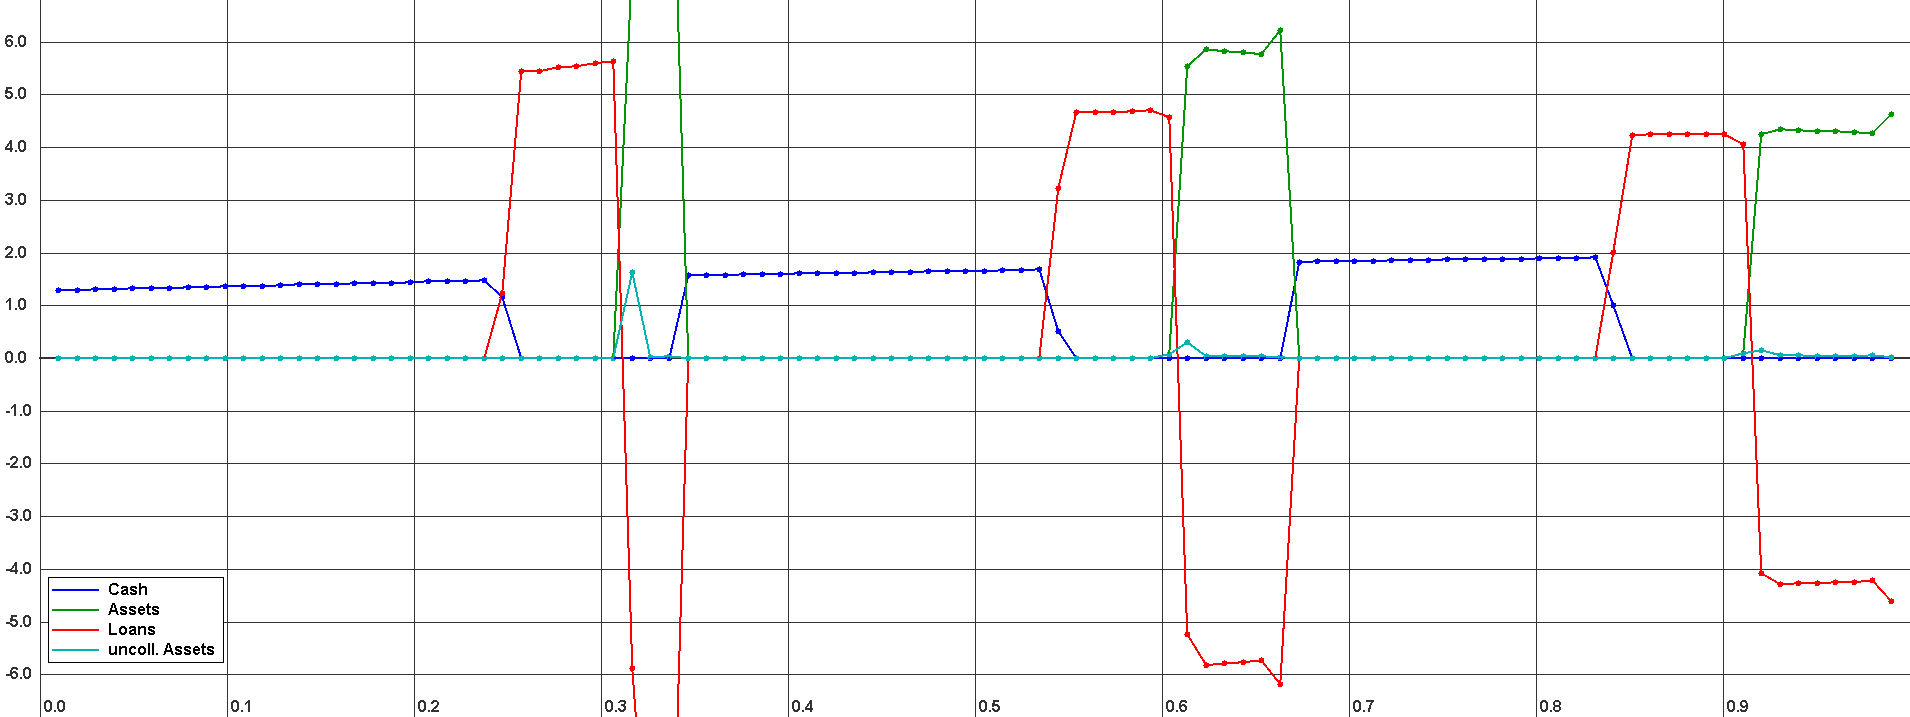
\includegraphics[width=1.0\textwidth, angle=0]{3HUBS_100_NOCOLLATERALMARKET_REPL.png}
	\caption{Wealth-Distribution of 3-Hubs topology}
	\label{fig:wealth_3HUBS_100_NOCOLLATERALMARKET_REPL}
\end{figure}

\subsection{1-Median Hub}
\begin{figure}[H]
	\centering
  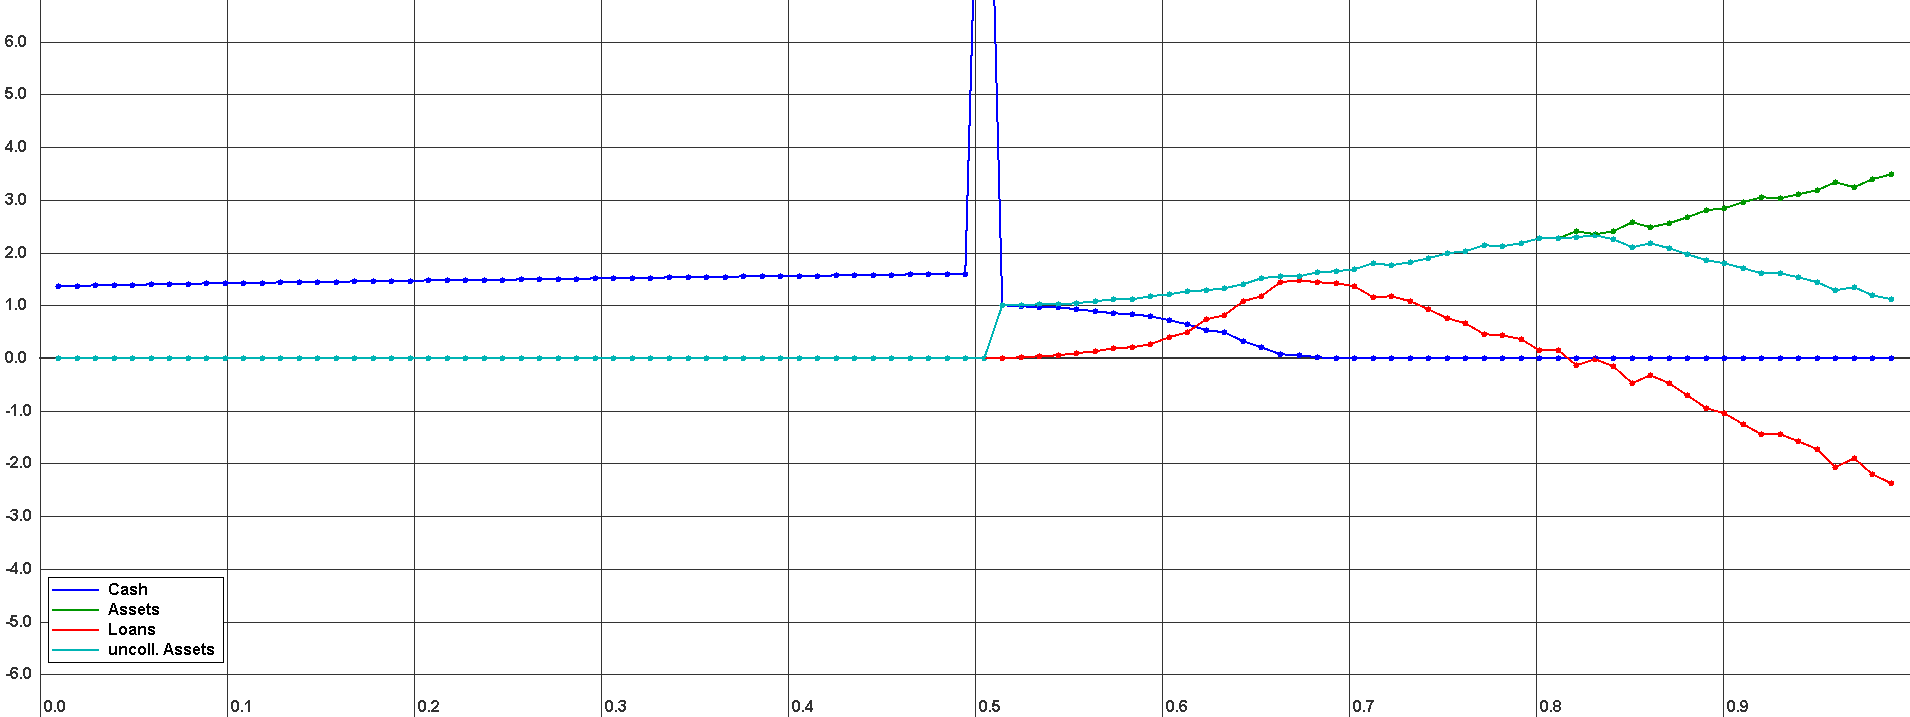
\includegraphics[width=1.0\textwidth, angle=0]{1MEDIANHUB_100_NOCOLLATERALMARKET_REPL.png}
	\caption{Wealth-Distribution of 1 Median-Hub topology}
	\label{fig:wealth_1MEDIANHUB_100_NOCOLLATERALMARKET_REPL}
\end{figure}

\subsection{3-Median Hubs}
\begin{figure}[H]
	\centering
  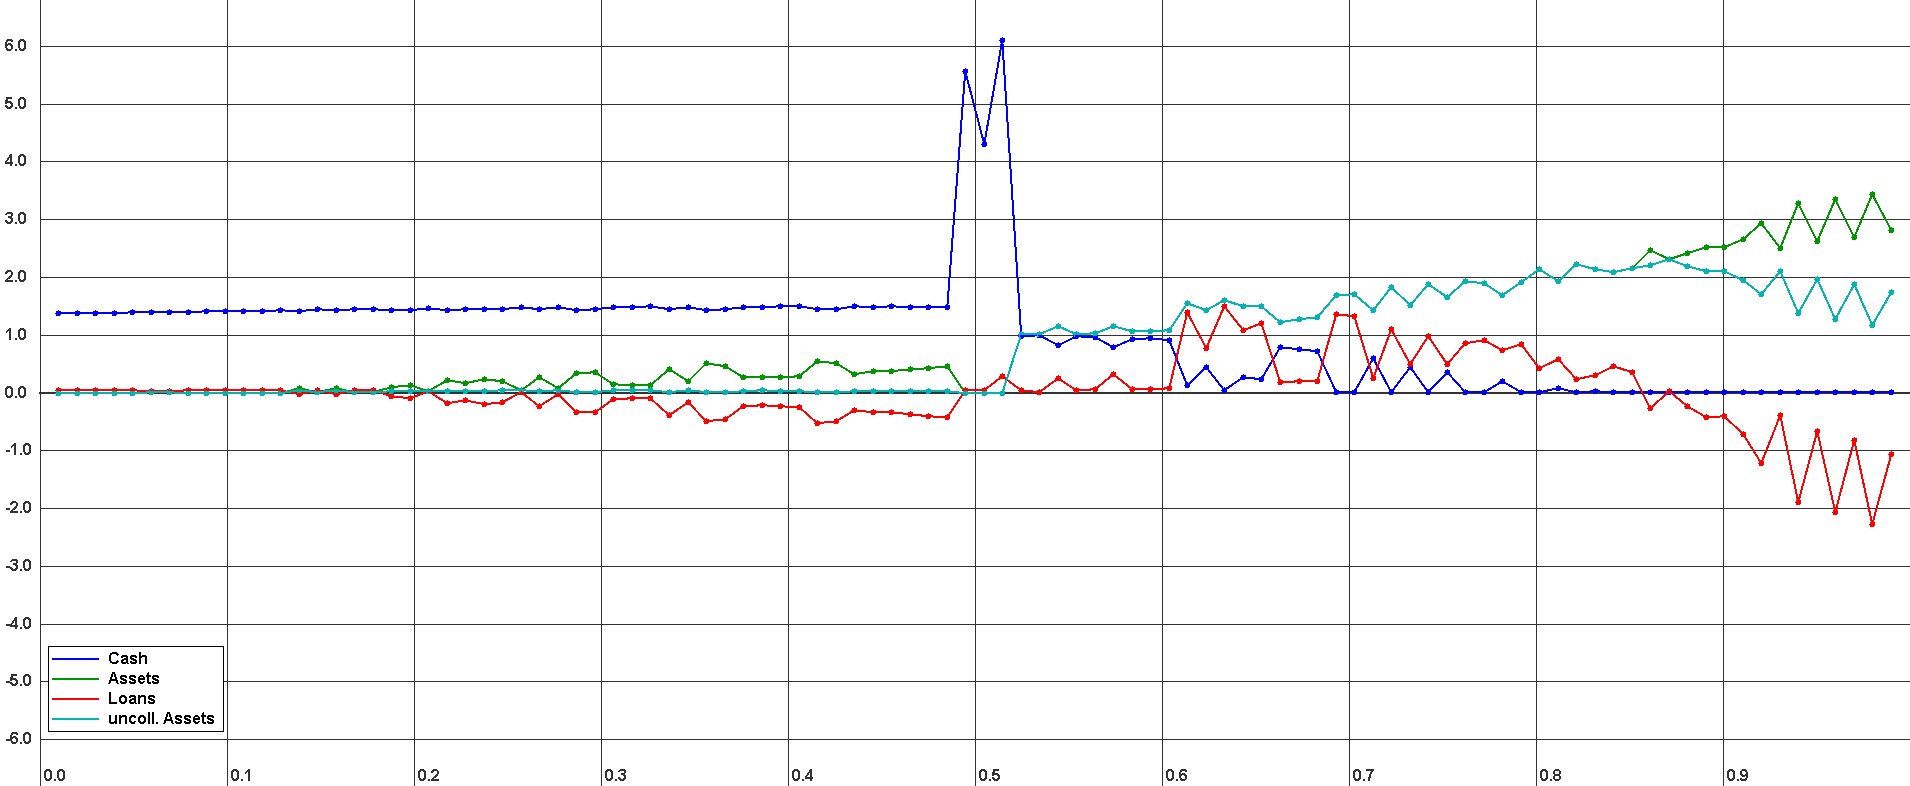
\includegraphics[width=1.0\textwidth, angle=0]{3MEDIANHUBS_100_NOCOLLATERALMARKET_REPL.png}
	\caption{Wealth-Distribution of 3 Median-Hubs topology}
	\label{fig:wealth_3MEDIANHUBS_100_NOCOLLATERALMARKET_REPL}
\end{figure}

\subsection{Maximum Hub}
\begin{figure}[H]
	\centering
  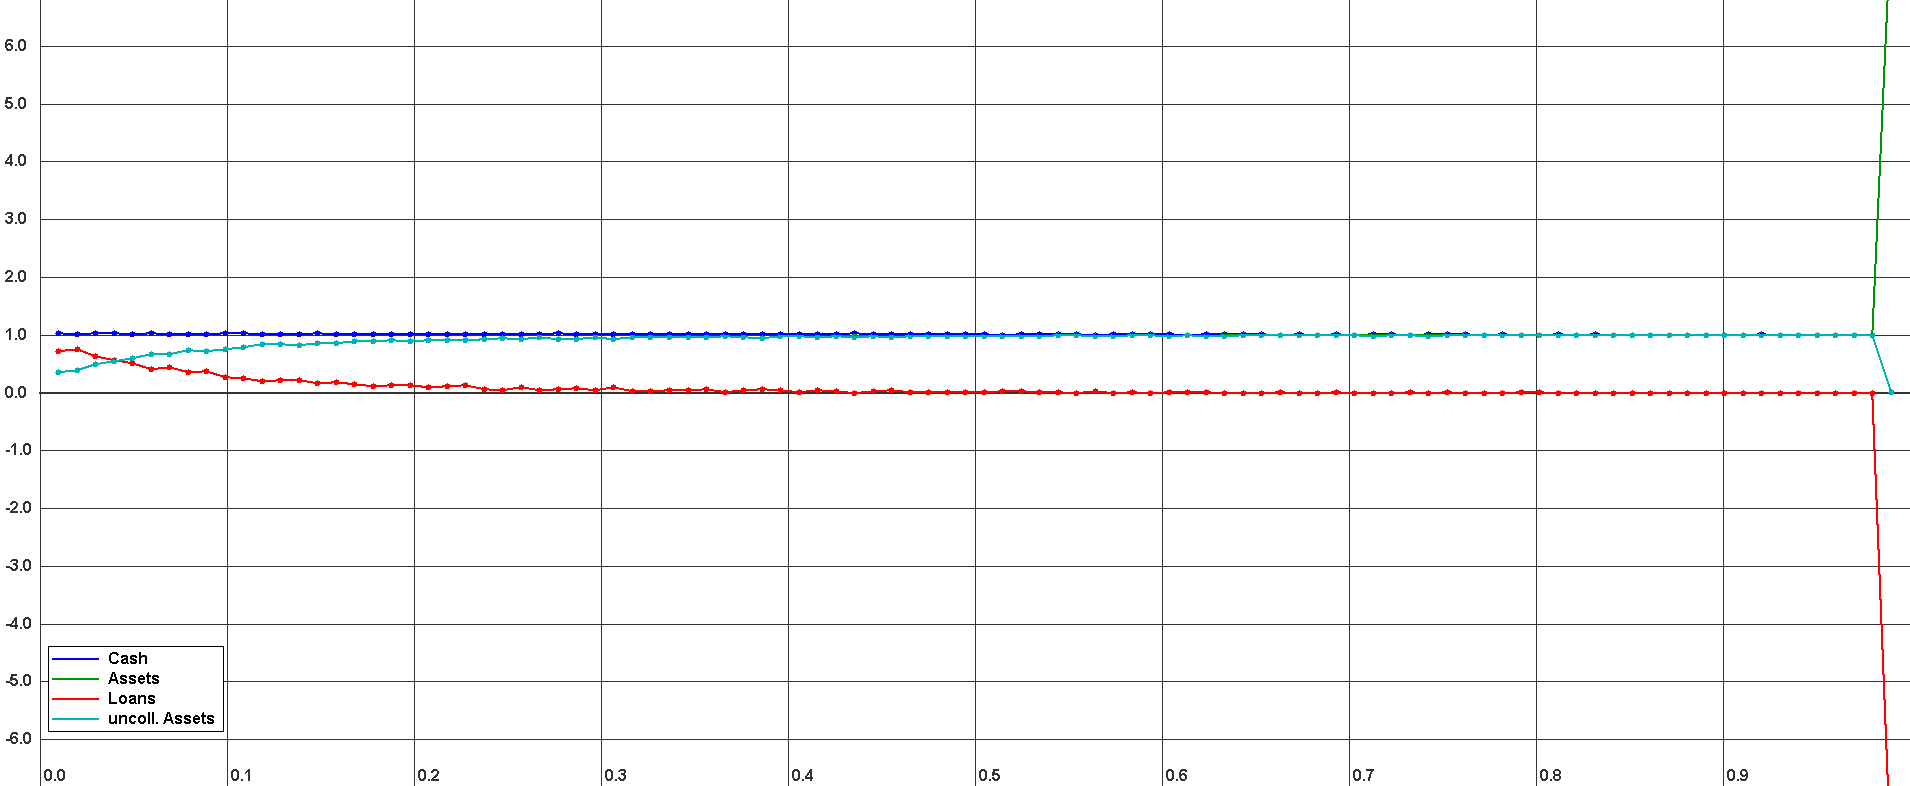
\includegraphics[width=1.0\textwidth, angle=0]{MAXIMUMHUB_100_NOCOLLATERALMARKET_REPL.png}
	\caption{Wealth-Distribution of Maximum-Hub topology}
	\label{fig:wealth_MAXIMUMHUB_100_NOCOLLATERALMARKET_REPL}
\end{figure}

\section{Scale-Free and Small-World topologies}
This topologies fail to come even close to equilibrium too due to reasons given in chapter \ref{ch:hypothesis} "Hypothesis". This can be seen also very clearly in the visual results and thus no performance- and equilibrium-tables are listed as they would not make any sense.

\subsection{Erdos-Renyi}
Note that with the correct parametrization this topology could satisfy the hypothesis by pure chance. The result would be a pure random network as an Ascending-Connected topology with random short-cuts but as already showed above this Ascending-Connected random short-cuts network fails from producing the theoretical and Fully-Connected equilibrium.

\begin{figure}[H]
	\centering
  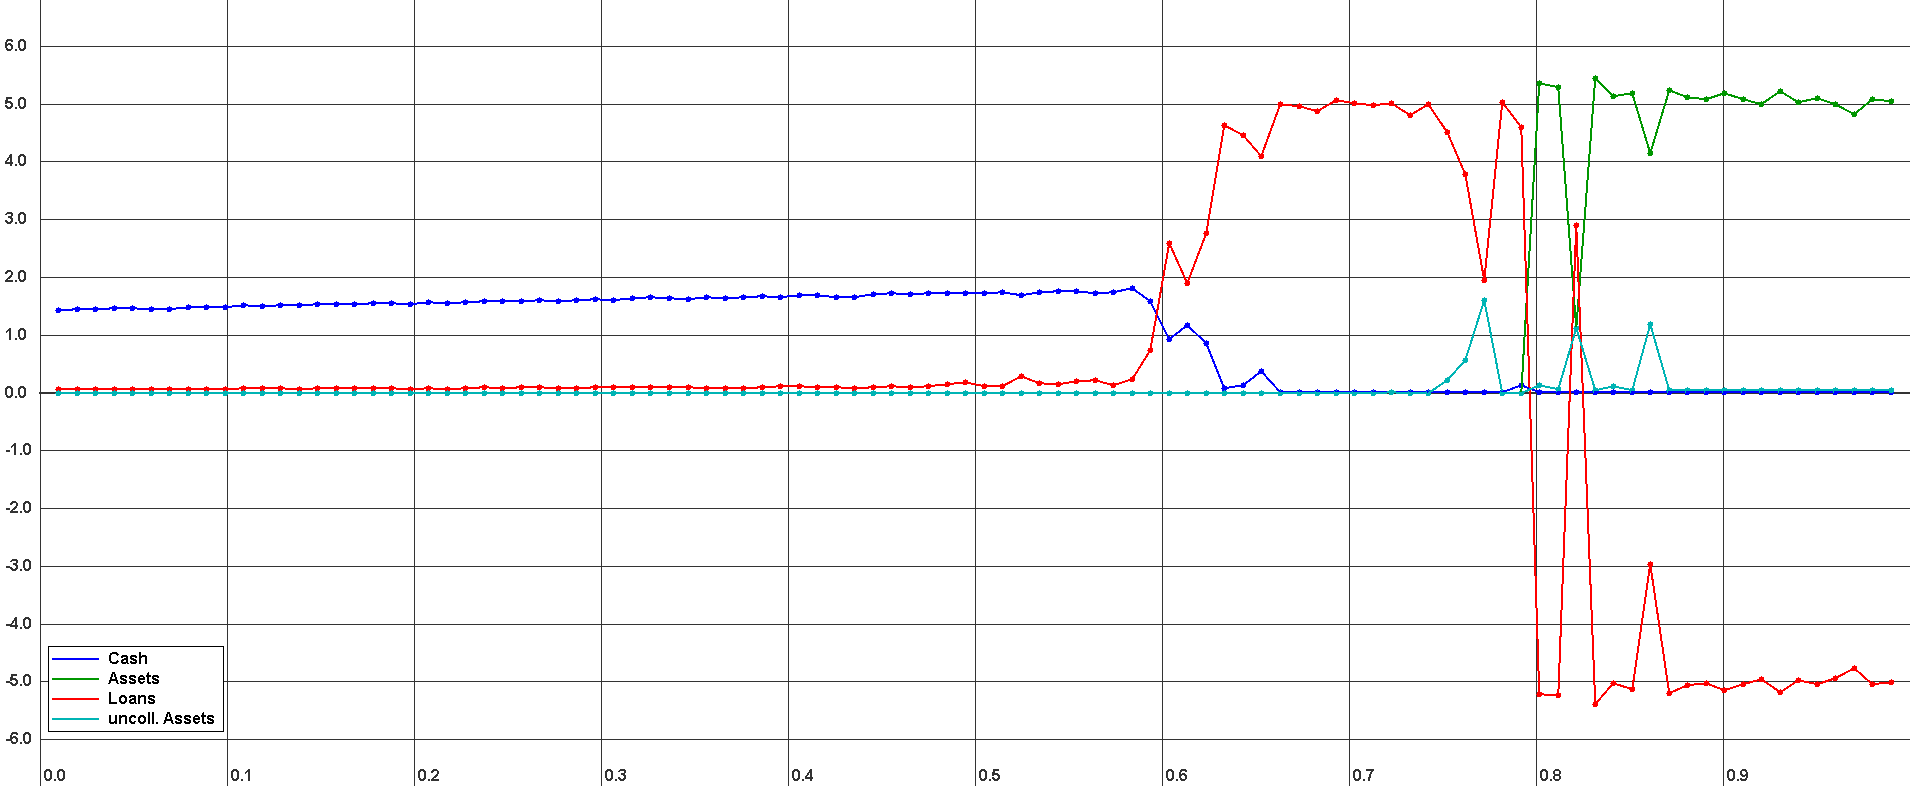
\includegraphics[width=1.0\textwidth, angle=0]{ERDOSRENYI_02_100_NOCOLLATERALMARKET_REPL.png}
	\caption{Wealth-Distribution of Erdos-Renyi 0.2 topology}
	\label{fig:wealth_ERDOSRENYI_02_100_NOCOLLATERALMARKET_REPL}
\end{figure}

\begin{figure}[H]
	\centering
  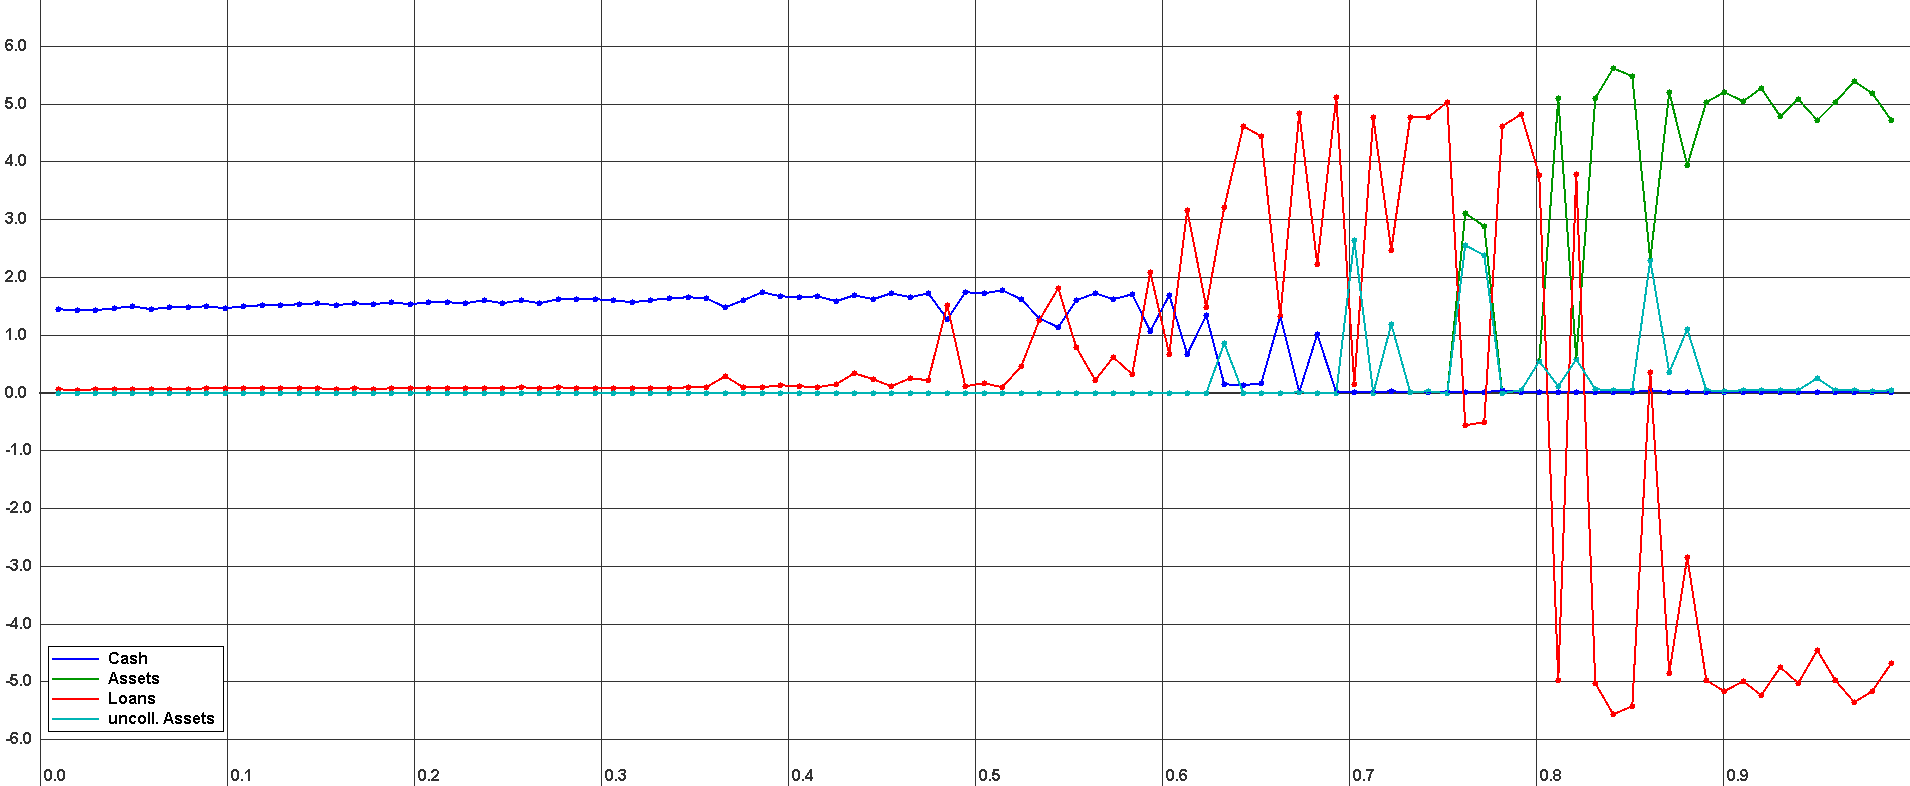
\includegraphics[width=1.0\textwidth, angle=0]{ERDOSRENYI_01_100_NOCOLLATERALMARKET_REPL.png}
	\caption{Wealth-Distribution of Erdos-Renyi 0.1 topology}
	\label{fig:wealth_ERDOSRENYI_01_100_NOCOLLATERALMARKET_REPL}
\end{figure}

\begin{figure}[H]
	\centering
  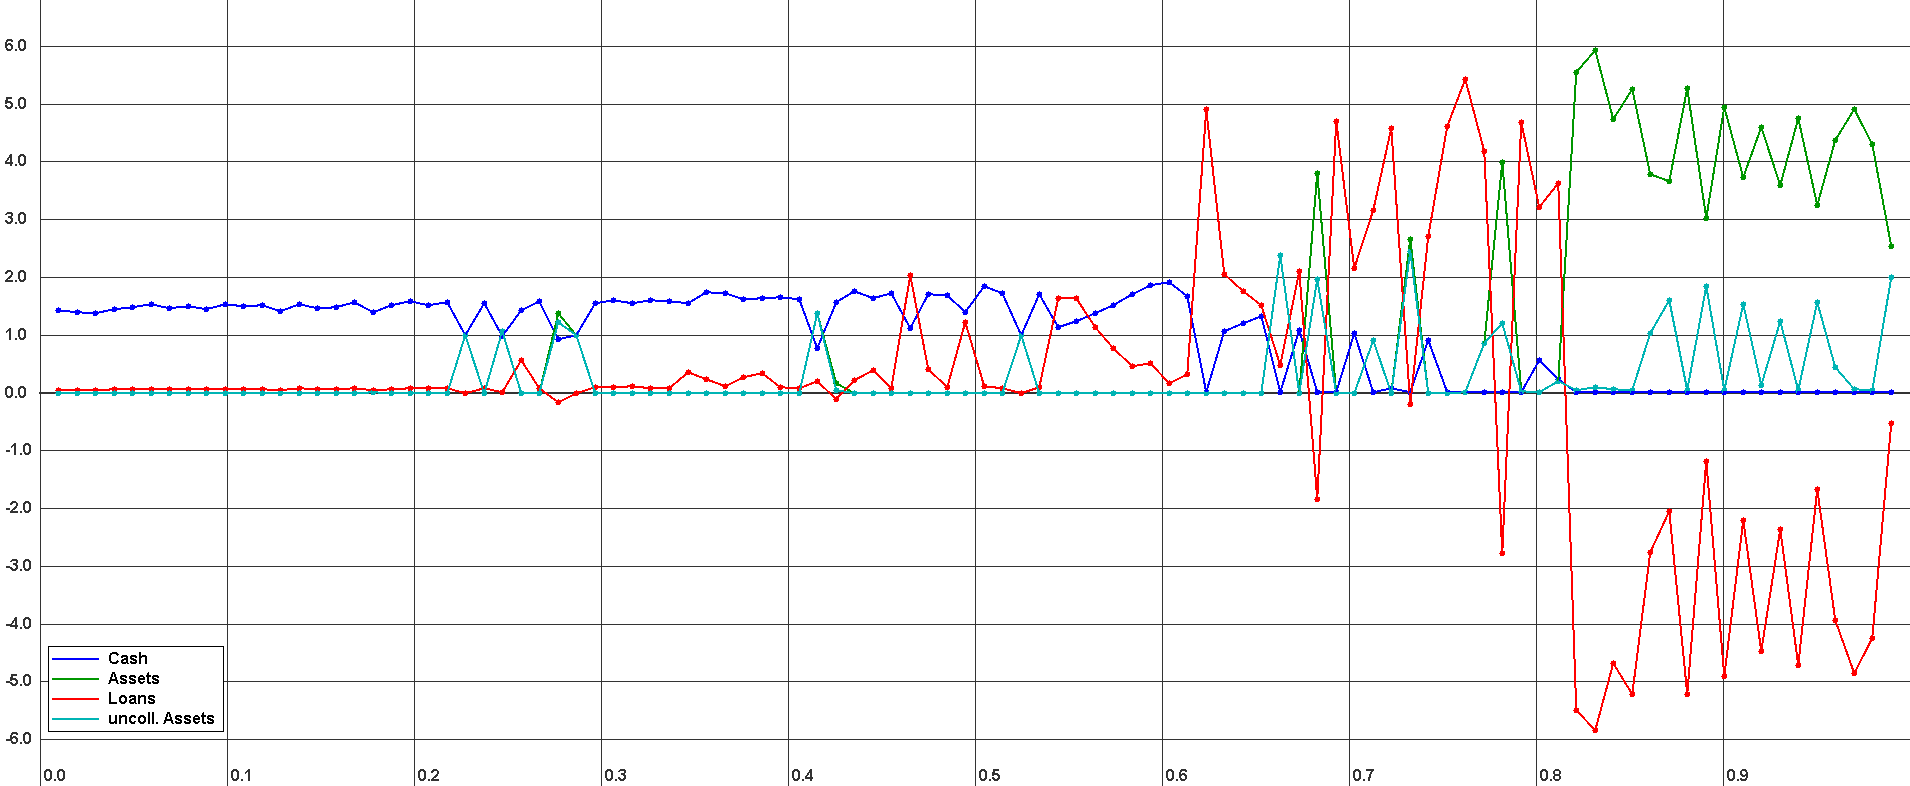
\includegraphics[width=1.0\textwidth, angle=0]{ERDOSRENYI_005_100_NOCOLLATERALMARKET_REPL.png}
	\caption{Wealth-Distribution of Erdos-Renyi 0.05 topology}
	\label{fig:wealth_ERDOSRENYI_005_100_NOCOLLATERALMARKET_REPL}
\end{figure}

\subsection{Barbasi-Albert}
\begin{figure}[H]
	\centering
  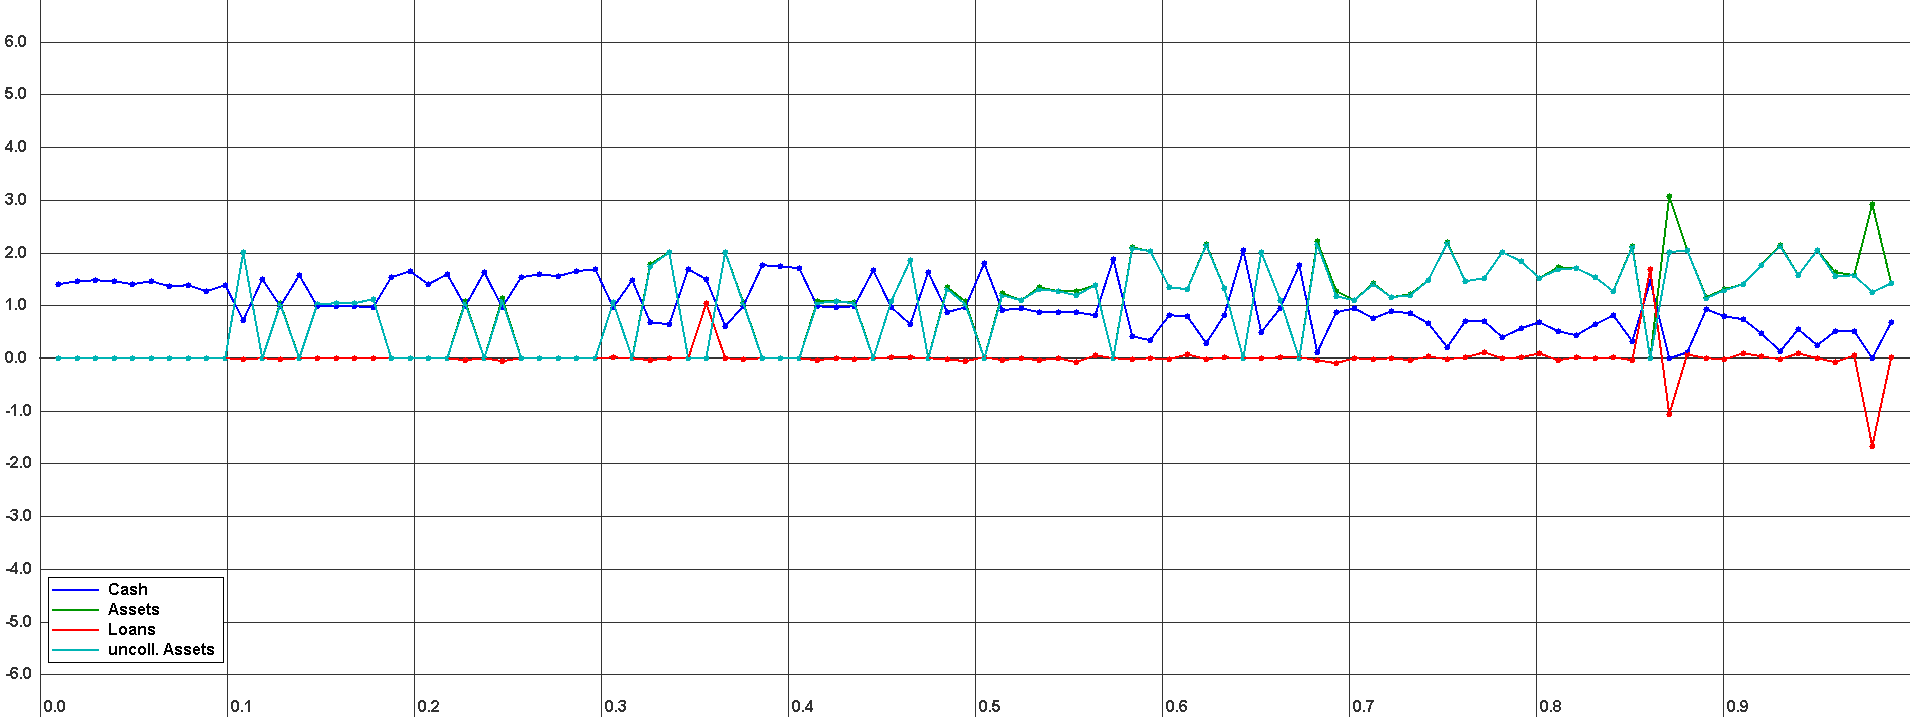
\includegraphics[width=1.0\textwidth, angle=0]{BARBASIALBERT_m03_m1_100_NOCOLLATERALMARKET_REPL.png}
	\caption{Wealth-Distribution of Barbasi-Albert m0=3, m=1 topology}
	\label{fig:wealth_BARBASIALBERT_m03_m1_100_NOCOLLATERALMARKET_REPL}
\end{figure}

\begin{figure}[H]
	\centering
  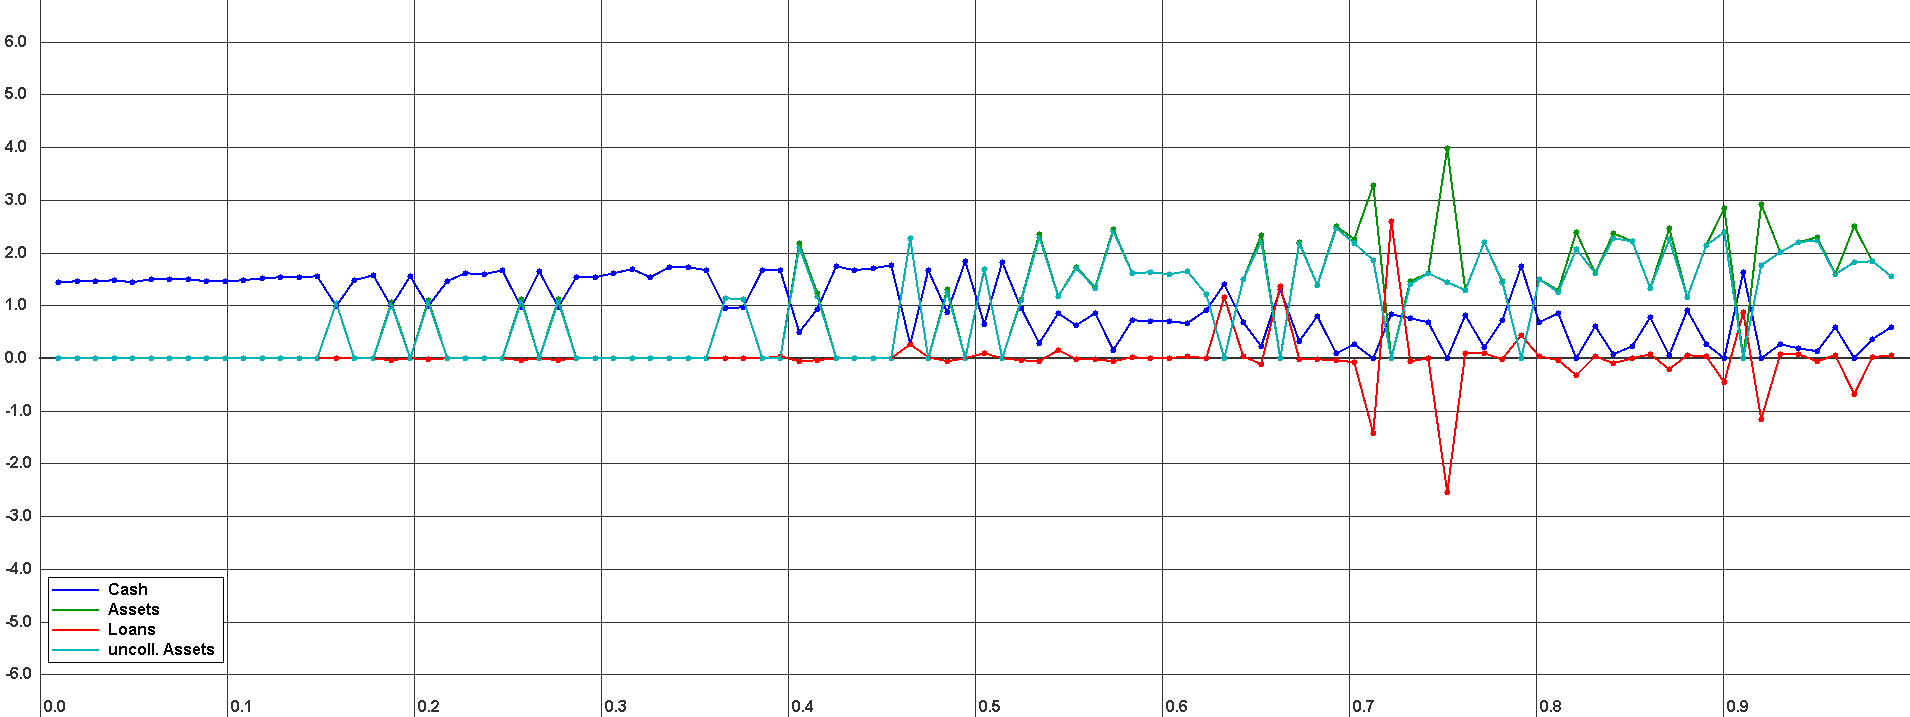
\includegraphics[width=1.0\textwidth, angle=0]{BARBASIALBERT_m09_m3_100_NOCOLLATERALMARKET_REPL.png}
	\caption{Wealth-Distribution of Barbasi-Albert m0=9, m=3 topology}
	\label{fig:wealth_BARBASIALBERT_m09_m3_100_NOCOLLATERALMARKET_REPL}
\end{figure}

\subsection{Watts-Strogatz}
Note that with the correct parametrization this topology could satisfy the hypothesis by pure chance too. The result would be a pure random network as an Ascending-Connected topology with random short-cuts but as already showed above this Ascending-Connected random short-cuts network fails from producing the theoretical and Fully-Connected equilibrium.

\begin{figure}[H]
	\centering
  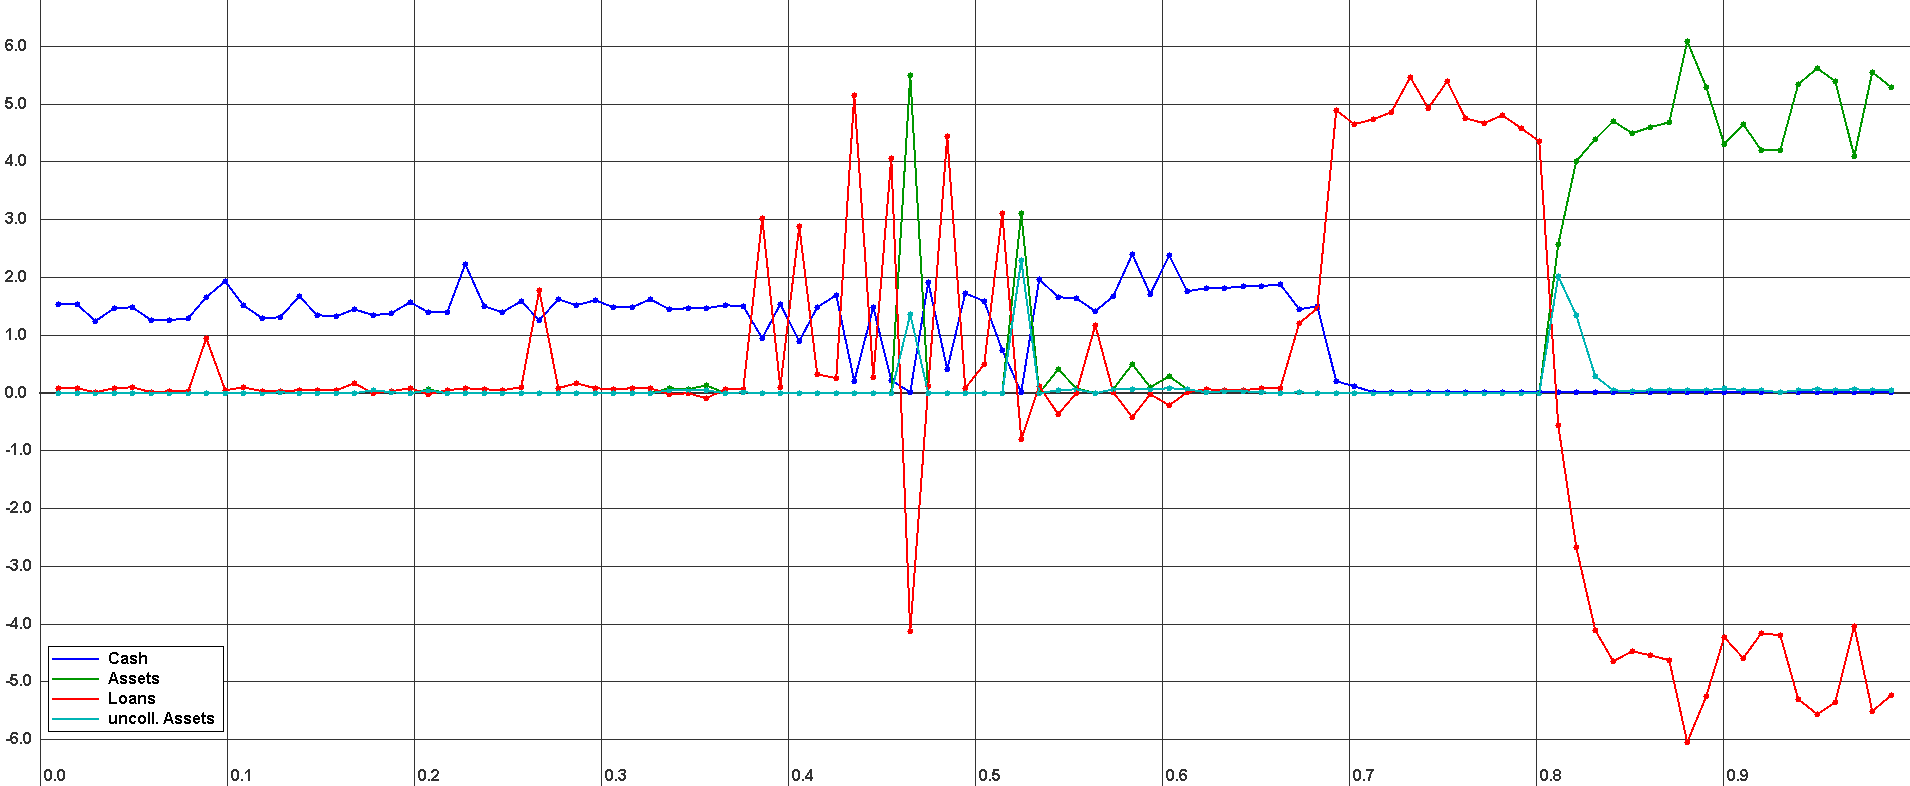
\includegraphics[width=1.0\textwidth, angle=0]{WATTSSTROGATZ_k2_b02_100_NOCOLLATERALMARKET_REPL.png}
	\caption{Wealth-Distribution of Watts-Strogatz k=2, b=0.2 topology}
	\label{fig:wealth_WATTSSTROGATZ_k2_b02_100_NOCOLLATERALMARKET_REPL}
\end{figure}

\end{document}
